\chapter{绪论}\label{chap:introduction}

随着信息技术的快速发展,人工智能、物联网等技术与智能终端的结合得越来越紧密,在智能终端上除了为用户提供基础服务以外还要提供更智能化的服务。因此,智能终端上要承担的计算任务越来越重。但目前智能终端上所拥有的计算、存储等资源并没有跟上对于智能终端计算能力的需求。与此同时,家庭、办公楼等智能终端环境中还存在着很多相对空闲、计算资源没有得到充分利用的计算设备。越来越重的计算任务与计算资源分配不均的矛盾日益凸显,为了解决这样的矛盾,在整体资源有限的情况下使资源利用达到最优化,我们想到可以使用多个智能终端协同提供服务,提供一种能够整合多终端资源、合理利用多终端资源的服务技术。

\section{研究背景}
% 这一段应该介绍的思路是:先介绍终端计算的发展、终端数量、计算能力的需求等待。然后介绍云计算和边缘计算相关。然后介绍虚拟化技术。

终端设备(Terminal Device)通常是指网络中能够对进行信息输入输出以及信息处理的节点\citep{2004支持普适计算的智能终端服务及设备管理技术研究}。在本研究中,智能终端设备主要指分布在用户身边的、具有一定计算能力的、能够进行网络连接和通信的、能够为用户提供计算服务的用户设备。随着信息技术的发展,智能终端设备的计算能力越来越强,设备规模越来越小,呈现智能化、轻量化、网络化的趋势。目前常见的智能终端设备包括智能手机、平板电脑、机顶盒、路由器、可穿戴设备、智能车、智能办公环境、智能家居环境等等。

在过去的几年中,智能终端设备通过提供按需的、弹性的、实时的、方便用户随时获取的移动服务,改变了传统计算服务的格局\citep{施巍松2017边缘计算}。智能手机、平板电脑、机顶盒、路由器等智能终端设备,正在逐渐成为人们现代数字化生活的重要组成部分。随着5G技术的日渐成熟以及物联网技术、边缘计算技术等技术的快速发展,万物互联的时代即将到来。根据中国信息通信研究院(工业和信息化部电信研究院)2016年的《物联网白皮书》预计,全球范围内的可穿戴设备、智能家电、自动驾驶汽车、智能机器人等新的智能设备接入物联网的数量将会达到数以百亿级,预计到2020年,全球联网设备数量将达到260亿个,物联网市场规模达到1.9万亿美元,全世界智慧城市总投资将达到1200亿美元\citep{物联网白皮书2016}。在未来的一段时间里,不仅智能终端设备的数量和规模大大增加,智能终端设备承担的计算任务也会越来越多,产生的数据量也会呈现爆炸式的增长。预计2020年,全球联网设备产生的总数据量将会达到44ZB\citep{物联网白皮书2016},智能终端设备的数据价值在不远的未来将会推动科技革命和工业革命的发展,并更进一步推动人们群众的生活方式向更智能化、数字化发展。

各种各样的新的信息技术在智能终端设备这样一个平台上的快速发展,在带来美好的技术变革的同时,也对智能终端设备的计算和存储能力提出了更高的要求。根据《思科全球云指数预测白皮书》的估计,2019年在网络边缘上的服务器、终端设备上所进行处理和计算的数据将会占全球物联网所产生的数据总量的45\%\citep{Cisco2016}。智能终端设备中央处理单元(CPU)的计算能力还不能跟上中断服务对其的要求\cite{dinh2013survey,othman2014survey,wang2015survey}。为了增强智能终端设备的计算和存储能力,提升智能终端服务质量,人们使用了云计算技术。云计算技术通过虚拟化技术,将云端的物理实体资源,包括计算、存储、内存、网络等资源进行虚拟化,形成资源池,可以让用户终端根据具体需求和费用考虑,灵活使用。云计算中的云端服务器拥有相对“无限”资源,通过网络提供给用户,帮助具有有限资源的智能终端设备执行需要更加强大的计算资源的复杂计算\citep{Noor.2018}。云计算是信息存储和处理的工业化过程, 是信息服务业的基础设施和服务平台\citep{江绵恒2010}。在不远的未来,云计算资源可以像水、电一样,通过水管、电线和网线进行传输,只需要打开开关就可以按需获取、按量计费,成为人们日常生活中和工业生产生活中可以随时随地获取的一种基础资源\citep{buyya2009cloud}。

尽管云计算能够大大增加智能终端设备的可用资源总量,但是面对呈现爆炸式增长趋势的智能终端数量以及智能终端待处理数据量,云计算的集中式处理模式仍然存着很多不足之处。云计算模式中的云数据处理中心(Data Center)距离用户的智能终端设备较远,传输时延较长,对于一些实时性较强的用户智能终端服务并不适合。海量的智能终端数据在网络上的传输也会造成带宽负载的浪费,大量的用户智能终端设备向云数据处理中心请求服务会造成网络的延迟和拥塞\citep{Ismail2016Evaluation}。另一方面,用户智能终端设备上产生的数据大多包含有用户个人隐私信息,在同云数据处理中心的数据通信过程中,存着极高的信息安全风险。

智能终端产生的海量数据,使得网络的传输能力和用户隐私安全问题成为限制万物互联时代快速发展的瓶颈,因此直接开发终端自身的潜能\citep{王劲林2015一种现场},利用智能终端自身的计算处理能力和智能终端之间短距离的局域网传输能力来对智能终端数据进行处理并提高智能终端服务质量成为一种可行的解决思路。在物联网中,智能设备除了作为数据源的作用外,还能够提供计算和存储功能,但是由于智能终端设备通常是专有目的的,可能只会使用几个小时,其他时间就空闲下来了\citep{renner2016towards}。由于用户智能终端设备总体数量庞大,因此还存在着大量的空闲资源没有得到充分利用,智能终端设备自身还有着很大的潜能可以开发利用。相比使用云计算技术中的云端资源来提供计算服务,使用智能终端设备来提供计算服务拥有很多优势。智能终端设备本身距离用户服务请求发起端更近,网络状态更好,传输时延短,服务响应更快,实时性更好。智能终端设备之间进行的局域网、短距离、高速度的传输,也能够大大减少对于公共网络带宽资源的占用,减少资源浪费。多个智能终端设备协同提供计算服务,用户的隐私数据只在内部传输,而不需要发送到很远的云端数据中心,这样面临的信息安全风险也大大降低。而且相比云计算的集中式模式,使用多智能终端协同提供计算服务能够,将智能终端大量的空闲资源利用起来,大大提高智能终端的资源利用率,减少智能终端资源浪费,而且其部署成本也更加低廉,可以直接利用现有智能终端设备,而不需要购买太多价格较为昂贵的独立服务器等设备,更不需要建立云计算模式中的云数据处理中心,部署成本较为低廉。

为了将智能终端设备上的资源加以管理和利用,我们参考云计算模式,引入了虚拟化技术。虚拟化技术能够将计算机或终端的资源如CPU、内存、存储等抽象、整合起来,打破实体资源的整体性,形成可以按需分配的资源池,让用户能够以更高效合理的方式来对智能终端资源进行管理和利用。传统的虚拟机(Virtual Machine,简称为VM)通常使用的是完全虚拟化技术,虚拟机启动时间非常长,也会消耗大量的额外资源来维持虚拟化功能。以Docker为代表的轻量级虚拟化技术近几年发展迅速,成为行业内最流行的解决方案。轻量级虚拟化技术利用基于Linux内核的LXC技术,可以以容器的形式将智能终端底层的物理实体资源按需封装起来,为用户提供服务,大大降低了对于智能终端上资源的管理和利用难度。可以说容器技术的快速发展,也是促成多智能终端协同服务技术成型的一个重要因素。

为了利用智能终端设备的潜力,还需要解决设备和应用的管理整合问题\citep{morabito2017evaluating}。本文研究了基于容器化的多智能终端协同服务技术,完成了一个多智能终端协同服务系统的架构设计,并着重研究了其中的几个模块,用来解决多智能终端协同技术中的设备、资源和应用的管理问题,提高智能终端设备的资源利用率,提高终端用户服务体验。



\section{研究意义}

随着信息技术的快速发展,未来智能终端设备可以成为一个获取互联网资源的入口,轻量级的自下而上的系统。

本研究针对智能终端计算任务越来越重与终端计算资源分布不均衡的问题,引入容器技术,对于多终端上的资源进行聚合管理,并通过多智能终端协同技术,合理分配利用终端空闲资源,提高智能终端的服务效率以及智能终端的资源利用率,为未来智能终端为用户提供日常生活服务以及与边缘计算、人工智能、物联网等技术的结合打下良好基础,具有重要的研究意义和应用价值。

% 本研究针对智能终端计算任务越来越重与终端计算资源分布不均衡的问题,引入容器技术,对于多终端上的资源进行聚合管理,并通过多智能终端协同技术,合理分配利用终端空闲资源,提高智能终端的服务效率以及智能终端的资源利用率,为未来智能终端为用户提供日常生活服务以及与边缘计算、人工智能、物联网等技术的结合打下良好基础,具有重要的研究意义和应用价值。

% 本研究针对智能终端计算任务越来越重与终端计算资源分布不均衡的问题,引入容器技术,对于多终端上的资源进行聚合管理,并通过多智能终端协同技术,合理分配利用终端空闲资源,提高智能终端的服务效率以及智能终端的资源利用率,为未来智能终端为用户提供日常生活服务以及与边缘计算、人工智能、物联网等技术的结合打下良好基础,具有重要的研究意义和应用价值。

基于以上现状,依托于中国科学院战略性先导科技专项课题,开展了基于容器化多终端协同服务技术研究,通过对基于容器化多终端协同服务系统架构的设计与研究,提高系统对于智能终端设备和终端服务应用的管理能力,并通过对基于容器的透明计算迁移技术的研究,提高系统对于智能终端计算资源的利用能力,通过研究多终端任务调度问题,提高了系统对于智能终端资源的利用率,最后通过研究基于预测的容器弹性服务问题,促进提高资源利用率和降低用户服务请求响应等待时间之间的平衡。本文的几个研究点相辅相成,最终目的是利用基于容器化的多终端协同服务技术,提高智能终端设备的资源利用率并提高终端服务的用户体验。

\section{研究内容}
为了解决终端计算能力跟不上以及终端空闲资源浪费的问题,我们研究多终端协同服务技术。引入了多终端协同技术和容器技术以后,整个系统会存在很多单一终端服务不会遇到的问题,例如多终端上的空闲资源如何使用、如何对多终端设备及其所提供的服务进行管理、如何提高智能终端设备的资源利用率、如何提高用户体验等待。本研究中主要通过研究四个方面来解决这些问题,包括基于容器化多终端服务系统架构设计、基于容器化的透明计算迁移技术、资源受限终端任务调度策略、基于预测的容器弹性服务策略。

本文针对上面提出的几个问题,首先介绍了边缘计算技术、容器虚拟化技术、计算迁移技术、任务调度算法、预测算法等相关技术和算法的研究现状,分析其目前还存在的问题。本文结合容器虚拟化技术和多终端协同服务技术,设计了基于容器化的多终端协同服务系统,并主要研究系统中的基于容器的多终端透明计算迁移技术、多终端协同服务任务调度算法优化以及基于预测的终端弹性服务技术。

本文具体研究内容如下:
\begin{enumerate}
    \item 随着计算机技术的快速发展和边缘计算技术的逐渐成熟,位于网络边缘的用户终端设备在用户的数字化生活中正扮演着越来越重要的角色,其定位逐渐从单一的用户服务发起者向用户服务的提供者转变。这会使用户终端承担越来越多的计算任务,这也对终端设备的服务质量和计算能力提出了越来越高的要求。但另一方面,边缘终端设备上还存在着大量没有得到充分利用的空闲资源。终端对计算能力要求越来越高与终端设备资源利用率不高之间存在着可以提升的空间,使用多终端协同服务技术来提升终端整体可用计算能力、提升终端整体资源利用率称为一种可行的方法。但是多终端协同服务技术还是会存着不少问题,如:终端资源管理、终端服务管理、多终端节点管理、节点组网等问题。为了解决这些问题,本文设计了基于容器化的多终端协同服务系统,引入容器虚拟化技术对多终端资源进行虚拟化,形成资源池,可以为上层终端服务按需使用;还参考微服务架构,提出多终端协同服务系统架构,可以进行终端服务管理;另外还提出了去中心化的自组织网络结构,进行多终端节点管理和节点组网。
    \item 相比云端协同计算,边缘终端设备距离用户更近,而且拥有很多空余资源没有得到充分利用,如何将这部分距离用户更近、成本更低的资源组织利用起来为用户设备提供计算迁移服务也成为了多终端协同服务技术中的一个值得研究的问题。为了将多终端上空闲的资源整合利用起来,为终端用户提供服务,提升用户体验,我们以HTML5中的Web Worker方法为例,研究Web应用透明计算迁移到以容器形式部署在边缘设备上的服务端,设计并实现了一种基于容器的Web Worker透明边缘计算迁移方法。一系列实验结果证明,所提出的方法能够将用户终端周围设备的空闲资源利用起来,为用户提供计算迁移服务,减少计算总执行时间,提高终端整体资源利用率,有效提高用户体验。
    \item 为了在终端资源有限且终端资源异构性极强的情况下,合理调度任务请求到更合适的执行节点上,使得任务总体开销更小,减少响应时间,提高用户体验,本研究基于一种群体智能的演进式优化算法————蝗虫优化算法,提出一种带有随机跳出机制的动态权重蝗虫优化算法来解决优化问题。在该算法中,我们在原有蝗虫优化算法的基础上,增加了基于完全随机跳出因素的跳出机制,来提高算法的跳出局部最优的能力。另外,我们还根据搜索阶段的不同,使用动态的权重参数来代替原算法中的线性递减搜索单元权重参数,帮助算法在不同的搜索阶段获得更大的迭代收益。经过一系列测试函数的实验验证,我们提出的带有随机跳出机制的动态权重蝗虫优化算法能够有效提高优化算法的搜索精度及收敛速度。在此基础上,我们进一步提出一种改进蝗虫优化算法,并将其应用于解决多终端任务调度问题。在该算法中,我们引入变型的sigmoid函数作为非线性舒适区调节参数,增强算法的搜索能力。同时,我们提出基于Levy飞行的局部搜索机制,让搜索单元在局部拥有一定的“搜索视觉”,提高算法的局部搜索能力。另外,我们还使用基于线性递减参数的随机跳出策略,增强算法跳出局部最优能力,并将成功跳出的结果影响力维持若干次迭代。经过一系列测试函数和标准测试集的实验,实验结果表明我们提出的改进蝗虫优化算法能够有效提高优化算法的搜索精度、稳定性、搜索到更优解的可能性及收敛速度。最后我们提出了终端上任务调度问题的数学模型,并将提出的改进蝗虫优化算法应用到该问题的求解过程中。实验结果证明,我们提出的改进蝗虫算法在求解终端上任务调度问题时能够得到很好的效果。
    \item 对于终端服务系统来说,如果不进行终端服务预部署,则当用户服务请求到达终端服务系统的时候现场启动基于Docker容器的终端服务端程序还是会消耗一定时间,尽管相比于传统的VM虚拟机,Docker容器技术的启动时间已经非常短了,但这个启动时间相比于用户请求等待响应时间仍然较长,不能接受。但是如果提前进行终端服务预部署,虽然可以达到缩短用户请求等待响应时间的目的,但是对于资源有限的终端来说,等待用户服务请求到达的过程会消耗大量额外的资源,同样是不能接受的。这就形成了一个矛盾的问题。为了解决是否进行预部署的问题,本研究提出了一种基于预测的容器弹性服务策略,利用改进的卡尔曼滤波算法,对未来一小段时间的用户请求流量进行预测,并根据预测结果对终端服务的容器规模进行适当调整,以达到在不增加用户请求响应等待时间、不降低用户体验的情况下对终端资源利用更合理的目的。经过一系列的仿真实验,证明所提出的基于预测的容器弹性服务策略能够有效根据用户请求流量的变化趋势动态调整终端服务规模,合理利用终端资源。
\end{enumerate}
\section{本文内容安排}
本文一共分为七个章节,针对基于容器化的多终端协同服务技术进行研究,组织结构如图\ref{fig:introduction_framework_of_organization}所示,各章节内容概述如下:
\begin{figure}[!htbp]
    \centering
    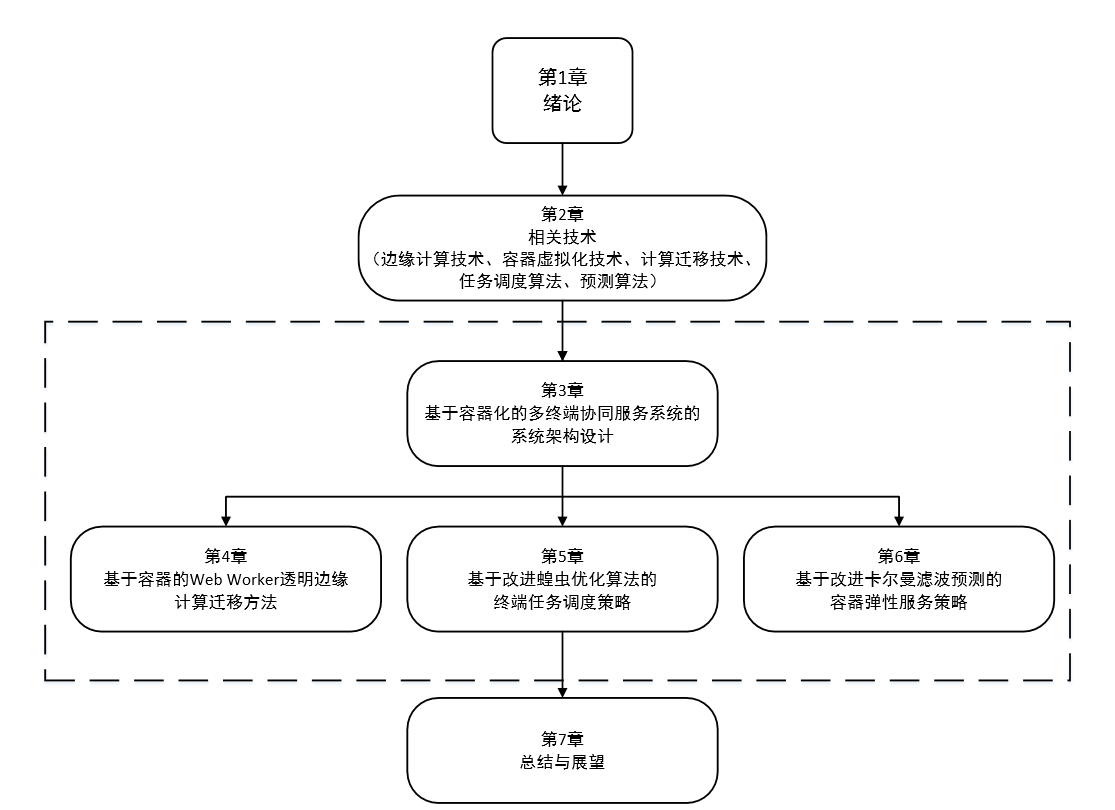
\includegraphics[width=1.0\textwidth]{Introduction_Framework_of_Organization_Temp}
    \caption{论文组织结构}
    \label{fig:introduction_framework_of_organization}
\end{figure}


第1章介绍了基于容器化的多终端协同服务技术的发展背景以及研究意义、本文的研究内容和本文内容安排。

第2章介绍了基于容器化的多终端协同服务技术的相关技术的研究现状,包括边缘计算技术、容器虚拟化技术、计算迁移技术、任务调度算法、预测算法等相关技术和算法。

第3章结合容器虚拟化技术和微服务架构,提出了基于容器化的多终端协同服务系统的系统架构设计及构建方法,解决了多终端节点管理、终端资源管理、终端服务管理等问题。后面三个研究点均为本章提出的系统中的部分具体实现。

第4章提出了一种基于容器的Web Worker透明边缘计算迁移方法,以透明计算迁移的方式将终端空闲资源利用起来为用户终端提供服务,减少任务计算执行时间,提高用户体验。

第5章提出了一种带有随机跳出机制的动态权重蝗虫优化算法来解决优化问题。并在此基础上提出了一种改进蝗虫优化算法,更进一步地提高了算法的性能,解决了终端任务调度问题。

第6章结合卡尔曼滤波算法,提出了一种基于预测的容器弹性服务策略,解决终端服务是否进行预部署的问题。

第7章总结了上述研究工作,并对未来工作进行了展望。
